% ------------------------------------------------------------------ %
% ESP Paper Template
% ------------------------------------------------------------------ %
% !TEX program = xelatex

%\documentclass{esp-paper} % Use this instead if ESP-only paper
\documentclass[external]{esp-paper}
\addbibresource{references.bib}

% ------------------------------------------------------------------ %
%  TITLE
% ------------------------------------------------------------------ %
\title{A Cross-Species Lexical Repertoire Enables Form-to-Meaning Translation in Animal Vocalizations}
\shorttitle{Cross-Species Lexical Repertoire}

% ------------------------------------------------------------------ %
%  AUTHORS
% ------------------------------------------------------------------ %
\author{Author~One$^{1\dagger\star}$}
\author{Author~Two$^{2\dagger\star}$}
\author{Author~Three$^{1\dagger}$}
\author{Author~Four$^{2\dagger}$}
\author{\authorcr Author~Five$^{1}$}
\author{Author~Six$^{1,2}$}

\affil{$^1$Earth Species Project}
\affil{$^2$External Institution}

% ------------------------------------------------------------------ %
%  CUSTOM COMMANDS
% ------------------------------------------------------------------ %
\newcommand{\dbname}{AnimalLex\xspace}
\newcommand{\nspecies}{57\xspace}
\newcommand{\ncalls}{373\xspace}

% ------------------------------------------------------------------ %
%  PACKAGES
% ------------------------------------------------------------------ %
\usepackage{xspace}
\usepackage{booktabs}

\begin{document}
\thispagestyle{firstpage}
\maketitle

% ------------------------------------------------------------------ %
%  FOOTER
% ------------------------------------------------------------------ %
\begingroup
\def\thefootnote{$\star$}\footnotetext{Corresponding author: \url{[PLACEHOLDER]@earthspecies.org}}
\def\thefootnote{$\dagger$}\footnotetext{These authors contributed equally to this work}
\def\thefootnote{\arabic{footnote}}
\endgroup

% ------------------------------------------------------------------ %
%  ABSTRACT
% ------------------------------------------------------------------ %
\begin{abstract}
	Understanding animal vocalizations requires connecting acoustic form to communicative meaning---a mapping that remains largely uncharted across the tree of life. We introduce \dbname, a curated cross-species repertoire database comprising \ncalls calls from \nspecies species spanning mammals, birds, and amphibians, annotated with standardized semantic and acoustic descriptions synthesized from the scientific literature and validated by domain experts. Using \dbname, we demonstrate three results. First, acoustic and semantic distances are significantly correlated both within and across species, providing evidence for conserved form-to-meaning structure that transcends phylogenetic boundaries. Second, models trained to predict semantic content from acoustic descriptions generalize across species and even across higher-level taxa, suggesting that this structure is learnable and systematic. Third, we leverage this structure to perform cross-species lexical translation: given any human concept, we identify its closest acoustic analogue in the animal kingdom, and conversely, we translate documented animal calls into human semantic terms. Together, these results suggest that a biological code linking acoustic form to communicative function may be a deep organizational principle of animal communication, and that large-scale repertoire curation unlocks new possibilities for comparative and translational bioacoustics.
\end{abstract}

% ------------------------------------------------------------------ %
%  BODY
% ------------------------------------------------------------------ %
\section{Introduction}

Animal communication spans an enormous range of acoustic and semantic complexity---from the stereotyped alarm calls of ground squirrels to the compositional songs of songbirds, from the long-distance rumbles of elephants to the rapid chirps of bats. Despite decades of study on individual species, no unified framework exists for comparing communicative systems across the tree of life. This gap impedes both basic science (we cannot ask whether convergent solutions to communicative problems are widespread) and applied goals (we cannot attempt translation between species).

A central unresolved question is whether the relationship between acoustic form and communicative meaning is arbitrary or systematic. In human language, the arbitrariness of the sign---the principle that the sound of a word bears no necessary relation to its meaning---is a classical tenet of structural linguistics \cite{saussure1916}. Yet counter-examples abound: sound symbolism, iconicity, and crosslinguistic tendencies for certain sound patterns to carry certain meanings suggest that arbitrariness is partial at best \cite{dingemanse2015arbitrariness}. In non-human animals, the question is even more open. Many alarm calls are short, broadband, and easily localizable---properties that plausibly reflect selection for rapid transmission and localization by conspecifics \cite{marler1955characteristics}. Infant contact calls tend to be high-pitched and repetitive across species---again, possibly reflecting shared physiological and evolutionary constraints. But whether these patterns constitute a widespread, learnable code connecting acoustic form to communicative function has not been tested systematically across species.

We address this question in three steps. First, we introduce \dbname, a curated dataset of \ncalls calls from \nspecies species (Figure~\ref{fig:dataset}), assembled by prompting large language models (LLMs) to extract and structure knowledge from the scientific literature, followed by expert validation. Each entry contains a structured semantic description (what the call communicates), a structured acoustic description (what the call sounds like), and standardized ontology keywords for both dimensions. Second, we use \dbname to test for form-to-meaning stability: we embed semantic and acoustic descriptions independently into vector spaces and ask whether their pairwise distance structures are correlated---within species, across species, and across higher taxa. Third, we use the resulting representations to perform lexical translation: for any human concept, we identify the closest animal vocalization, and for any documented call, we identify its closest human semantic analogue.

Our results provide evidence that form-to-meaning mapping is not arbitrary across the animal kingdom. Acoustic and semantic spaces are aligned in a way that is learnable, generalizable, and meaningful enough to support translation. This opens a new paradigm for comparative bioacoustics: rather than studying communication system by system, we can leverage the accumulated knowledge of the field---as compressed by LLMs---to ask questions at the scale of the tree of life.

\section{Dataset: \dbname}

\subsection{Collection and curation}

\dbname was constructed in two stages. In the first stage, we prompted a large language model (GPT-4o; \citealt{openai2024gpt4}) to synthesize knowledge from the primary scientific literature for each target species, producing structured entries containing: (1) the call name, (2) a free-text acoustic description, (3) a free-text semantic description, (4) a set of standardized ontology keywords for the semantic content, (5) a subjective reliability rating, and (6) primary literature references. The LLM was instructed to restrict itself to documented, peer-reviewed findings and to flag uncertain or contested claims. In the second stage, domain experts reviewed all entries, corrected errors, added missing calls, and updated reliability ratings. The final dataset contains \ncalls calls from \nspecies species.

Species were selected to maximize taxonomic breadth and the availability of primary-literature evidence. The dataset covers \nspecies species across three vertebrate classes: 43 mammals (Mammalia), 9 birds (Aves), and 5 amphibians (Amphibia). Mammalian species include African savanna elephants (\textit{Loxodonta africana}), gray wolves (\textit{Canis lupus}), Egyptian fruit bats (\textit{Rousettus aegyptiacus}), and meerkats (\textit{Suricata suricatta}), among others. Avian species include the Carolina chickadee (\textit{Poecile carolinensis}), the Japanese tit (\textit{Parus minor}), and the Bengalese finch (\textit{Lonchura striata domestica}). Amphibian species include the t\'{u}ngara frog (\textit{Engystomops pustulosus}) and the American bullfrog (\textit{Lithobates catesbeianus}).

\subsection{Dataset statistics}

\begin{figure}[t]
	\centering
	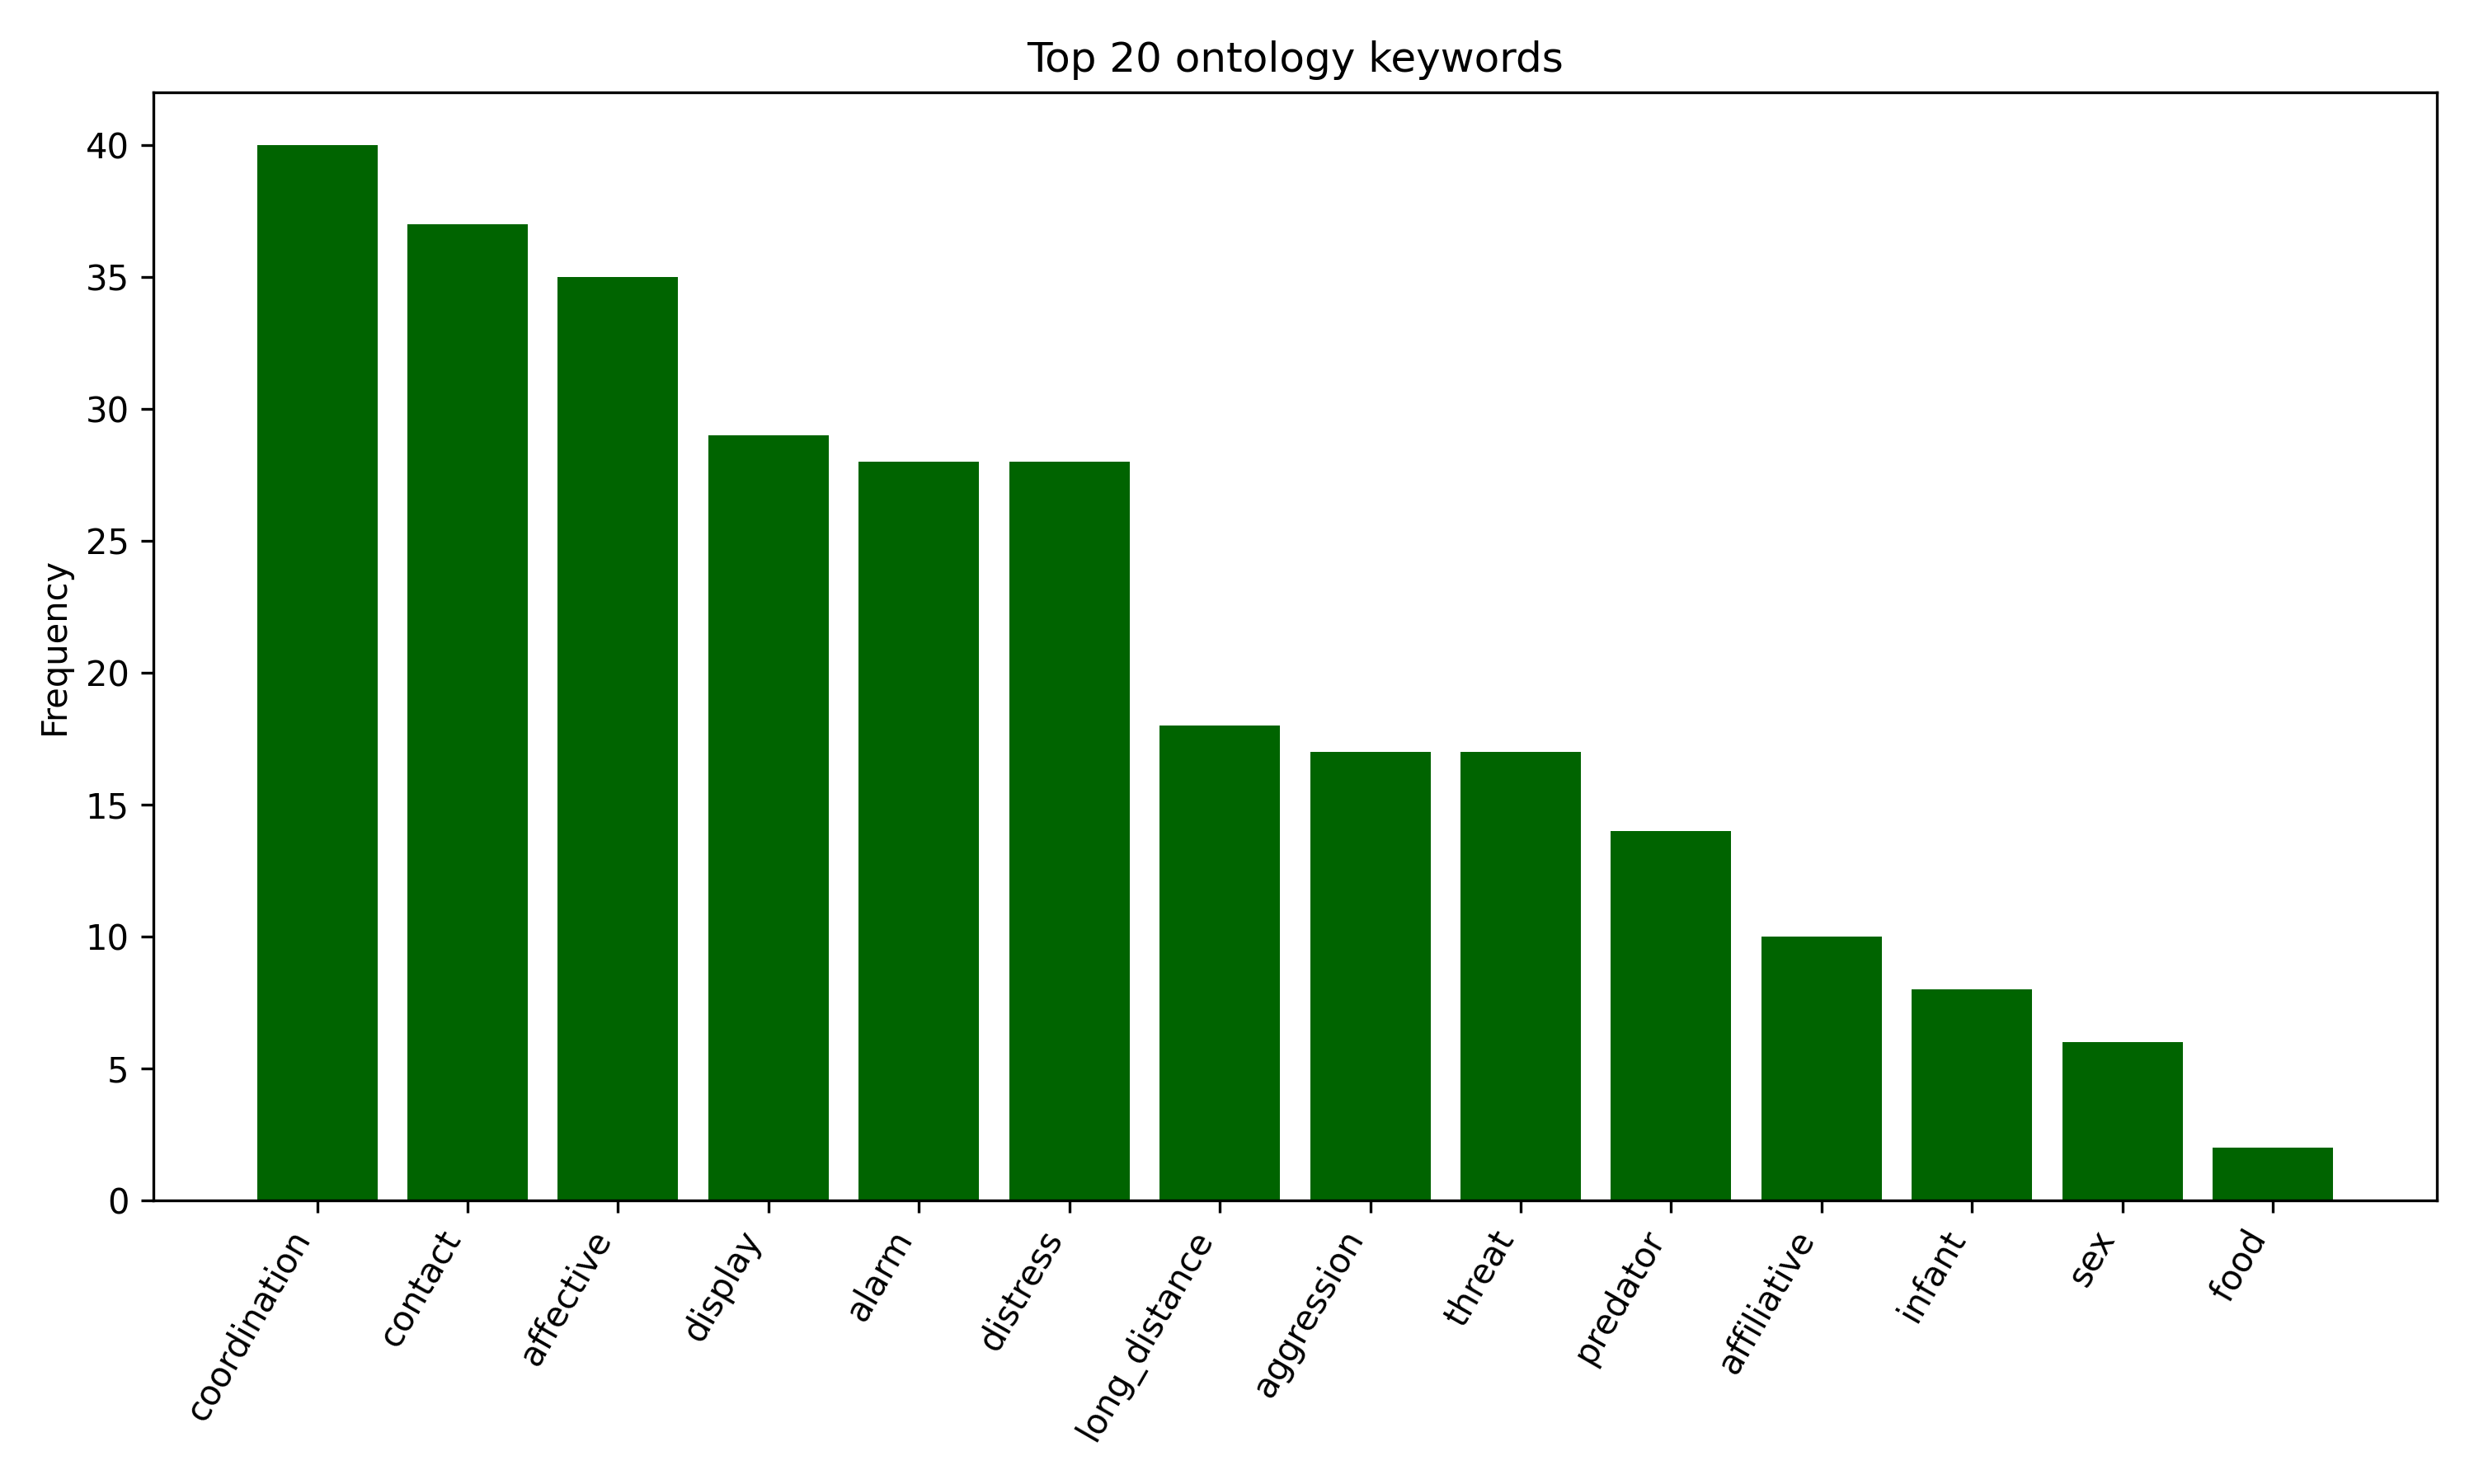
\includegraphics[width=\textwidth]{../plots/keyword_freq.png}
	\caption{\textbf{\dbname dataset overview.} (\textbf{A}) Distribution of semantic ontology keywords across all \ncalls calls in \dbname, colored by broad communicative category. The most frequent categories are coordination, contact, alarm, and affective signaling. (\textbf{B}) Distribution of acoustic description keywords [placeholder: requires acoustic keyword extraction]. (\textbf{C}) Taxonomic breakdown of species in the database. (\textbf{D}) Number of calls per species, showing the range from small repertoires (3--4 calls) to larger ones (10+ calls).}
	\label{fig:dataset}
\end{figure}

The \ncalls calls in \dbname span a wide range of communicative functions. The most frequent semantic categories are coordination (n=106 calls), affective signaling (n=98), contact and cohesion (n=94), distress (n=72), and alarm (n=71; Figure~\ref{fig:dataset}A). Less frequent but scientifically important categories include referential signaling (n=5), individual identity coding (n=8), and learning-related calls (n=10). This distribution reflects both the taxonomic composition of the database and genuine differences in how thoroughly different communicative functions have been studied.

On the acoustic side, descriptions in \dbname capture a wide range of spectro-temporal features: frequency range and modulation, temporal structure (pulsed vs.\ tonal, rhythm, duration), amplitude envelope, and call-internal structure (notes, syllables, phrases). These descriptions provide a rich substrate for asking whether acoustic properties covary systematically with semantic content.

\subsection{Semantic and acoustic embedding spaces}

\begin{figure}[t]
	\centering
	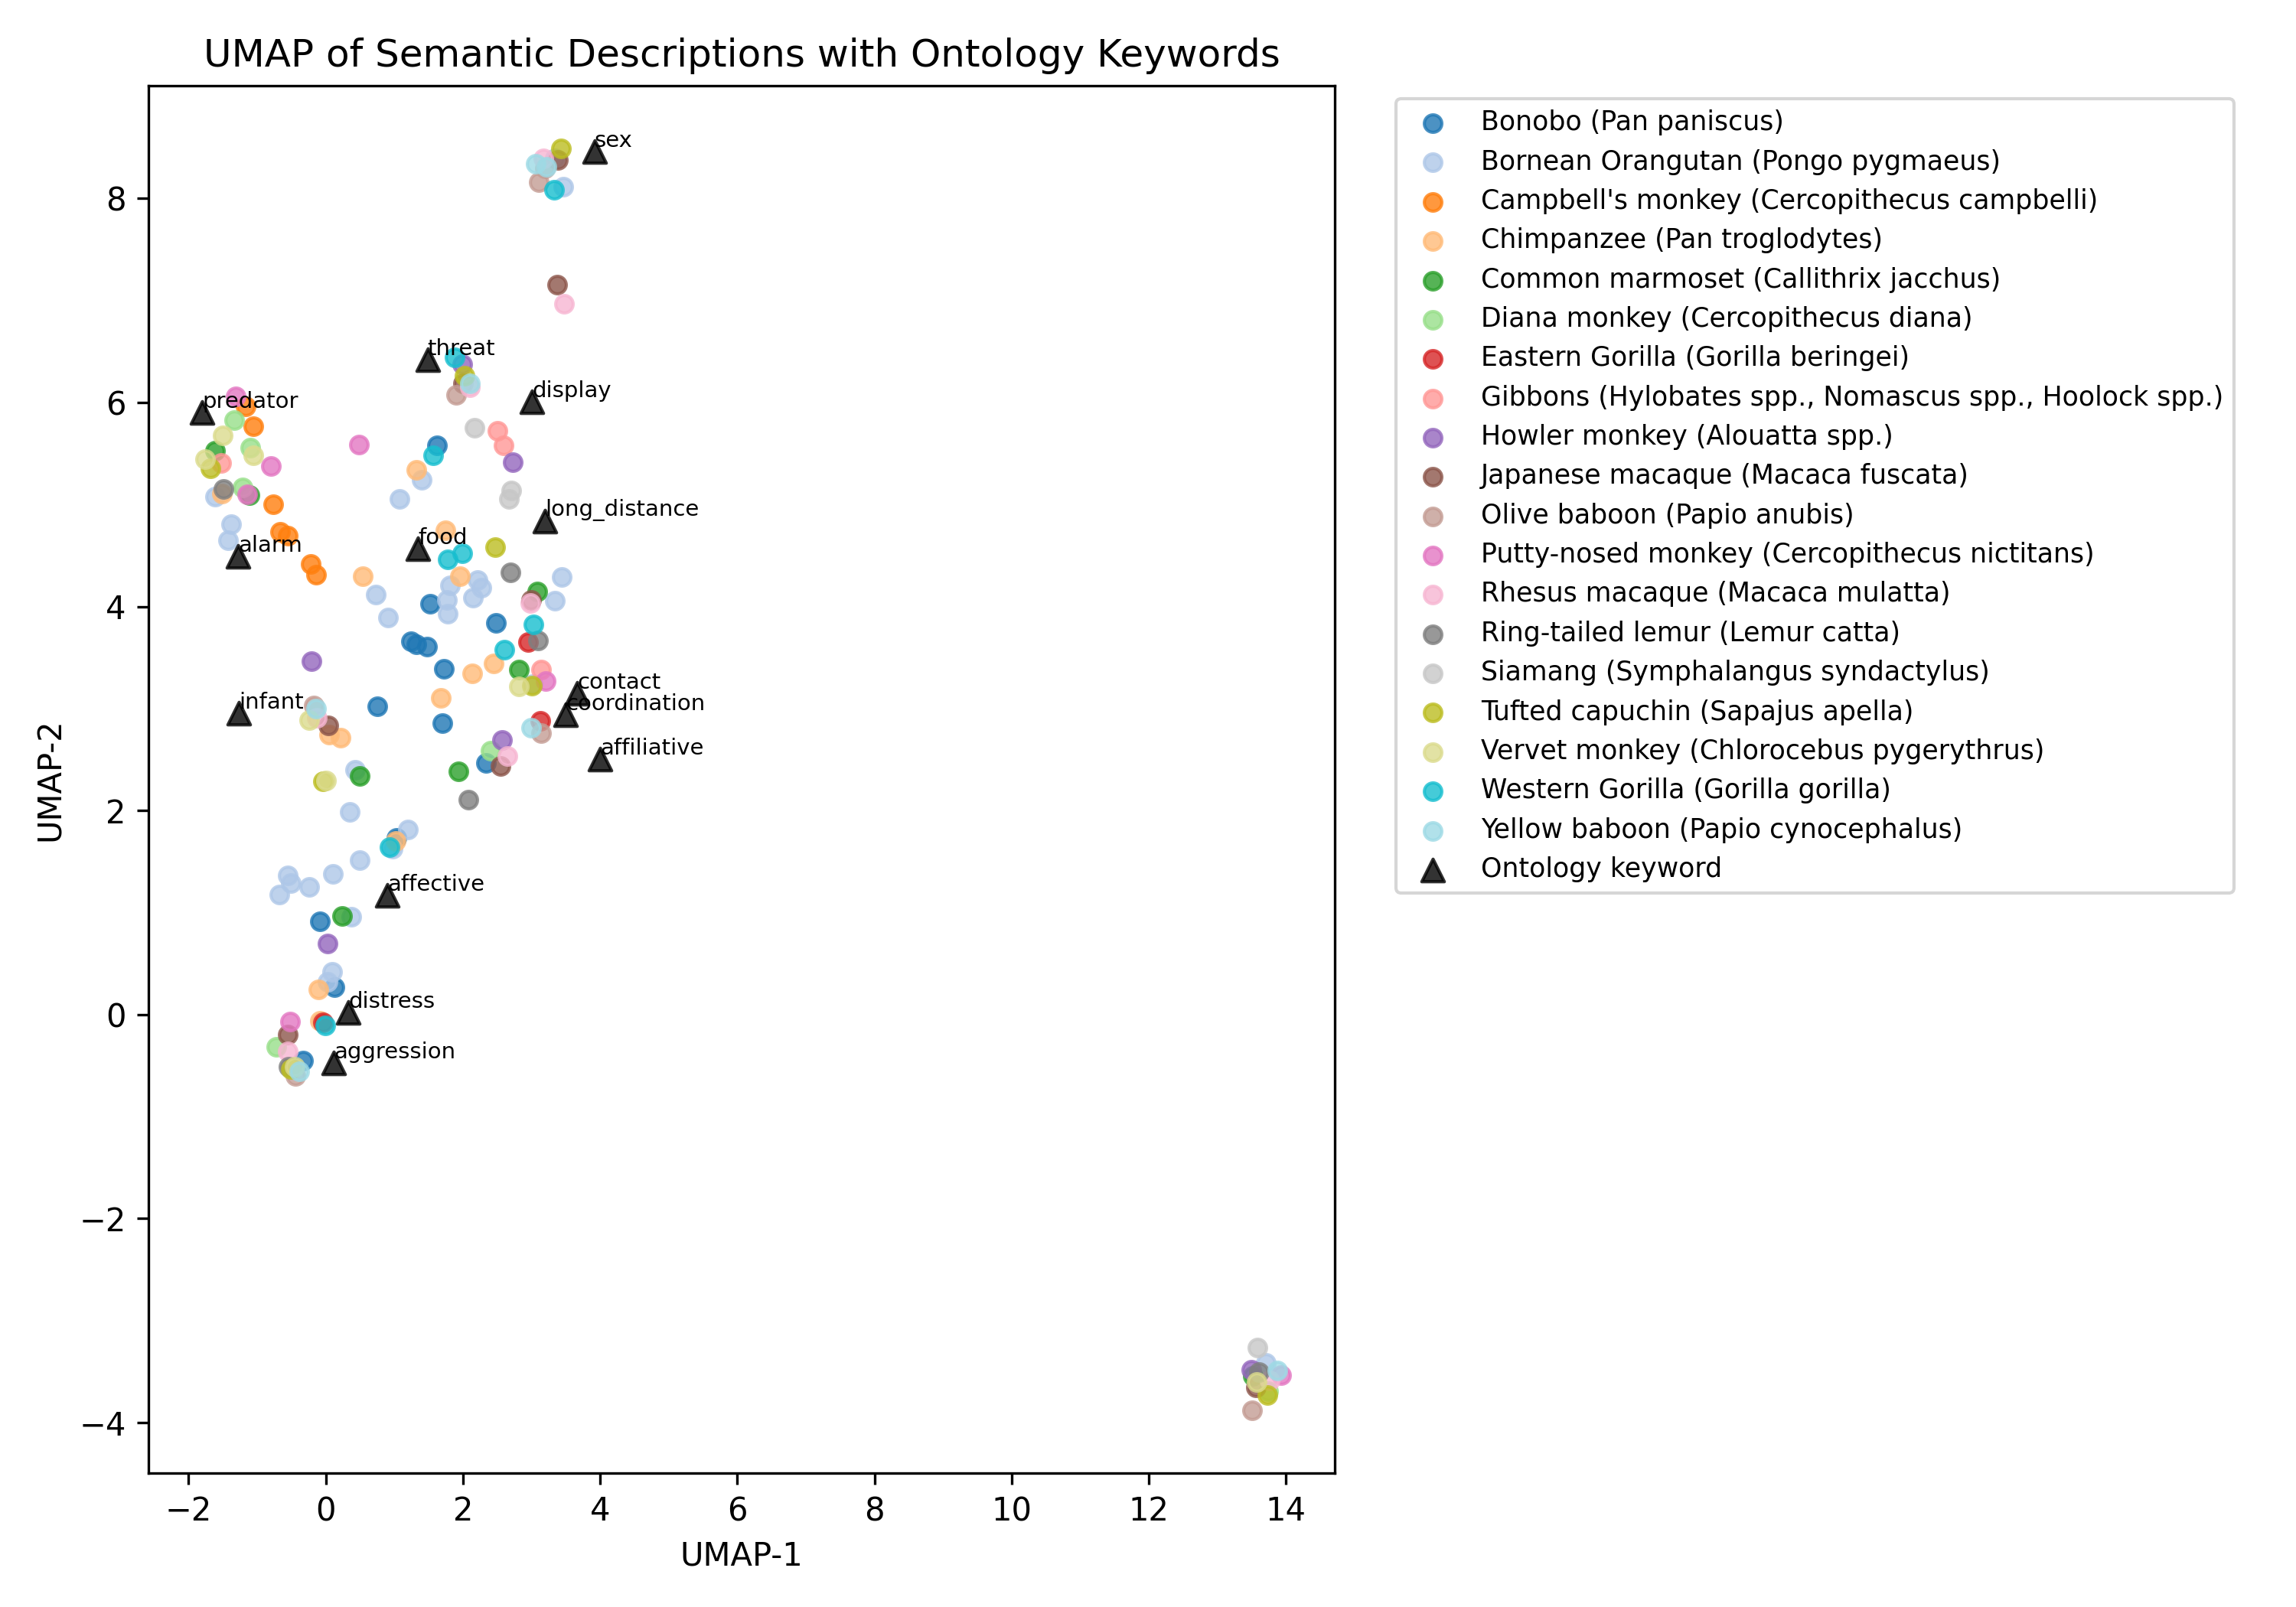
\includegraphics[width=\textwidth]{../plots/semantic_umap.png}
	\caption{\textbf{Semantic and acoustic embedding spaces.} UMAP projections of (\textbf{A}) semantic and (\textbf{B}) acoustic embeddings of all calls in \dbname, colored by ontology keyword category. Calls with similar meanings cluster together in semantic space, and calls with similar acoustic properties cluster together in acoustic space. The degree to which these two clusterings align is the subject of Results 1--2.}
	\label{fig:embeddings}
\end{figure}

To analyze form-to-meaning relationships, we embedded both semantic and acoustic descriptions into continuous vector spaces using a pre-trained sentence transformer (all-MiniLM-L6-v2; \citealt{reimers2019sentence}). Semantic embeddings were derived from the free-text semantic descriptions; acoustic embeddings were derived from the free-text acoustic descriptions. Figure~\ref{fig:embeddings} shows UMAP projections of both spaces. In semantic space, calls with related functions---alarms, contact calls, infant-directed calls---form coherent clusters. In acoustic space, calls described in similar terms (tonal, high-frequency; broadband, pulsed) similarly cluster. Whether these two spaces are aligned is tested in Results 1 and 2 below.

\section{Result 1: Form-to-meaning stability---correlational evidence}

\subsection{Acoustic distance predicts semantic distance}

\begin{figure}[t]
	\centering
	% placeholder figure: scatter plot of acoustic vs. semantic distance, Mantel test results, by phylogenetic level
	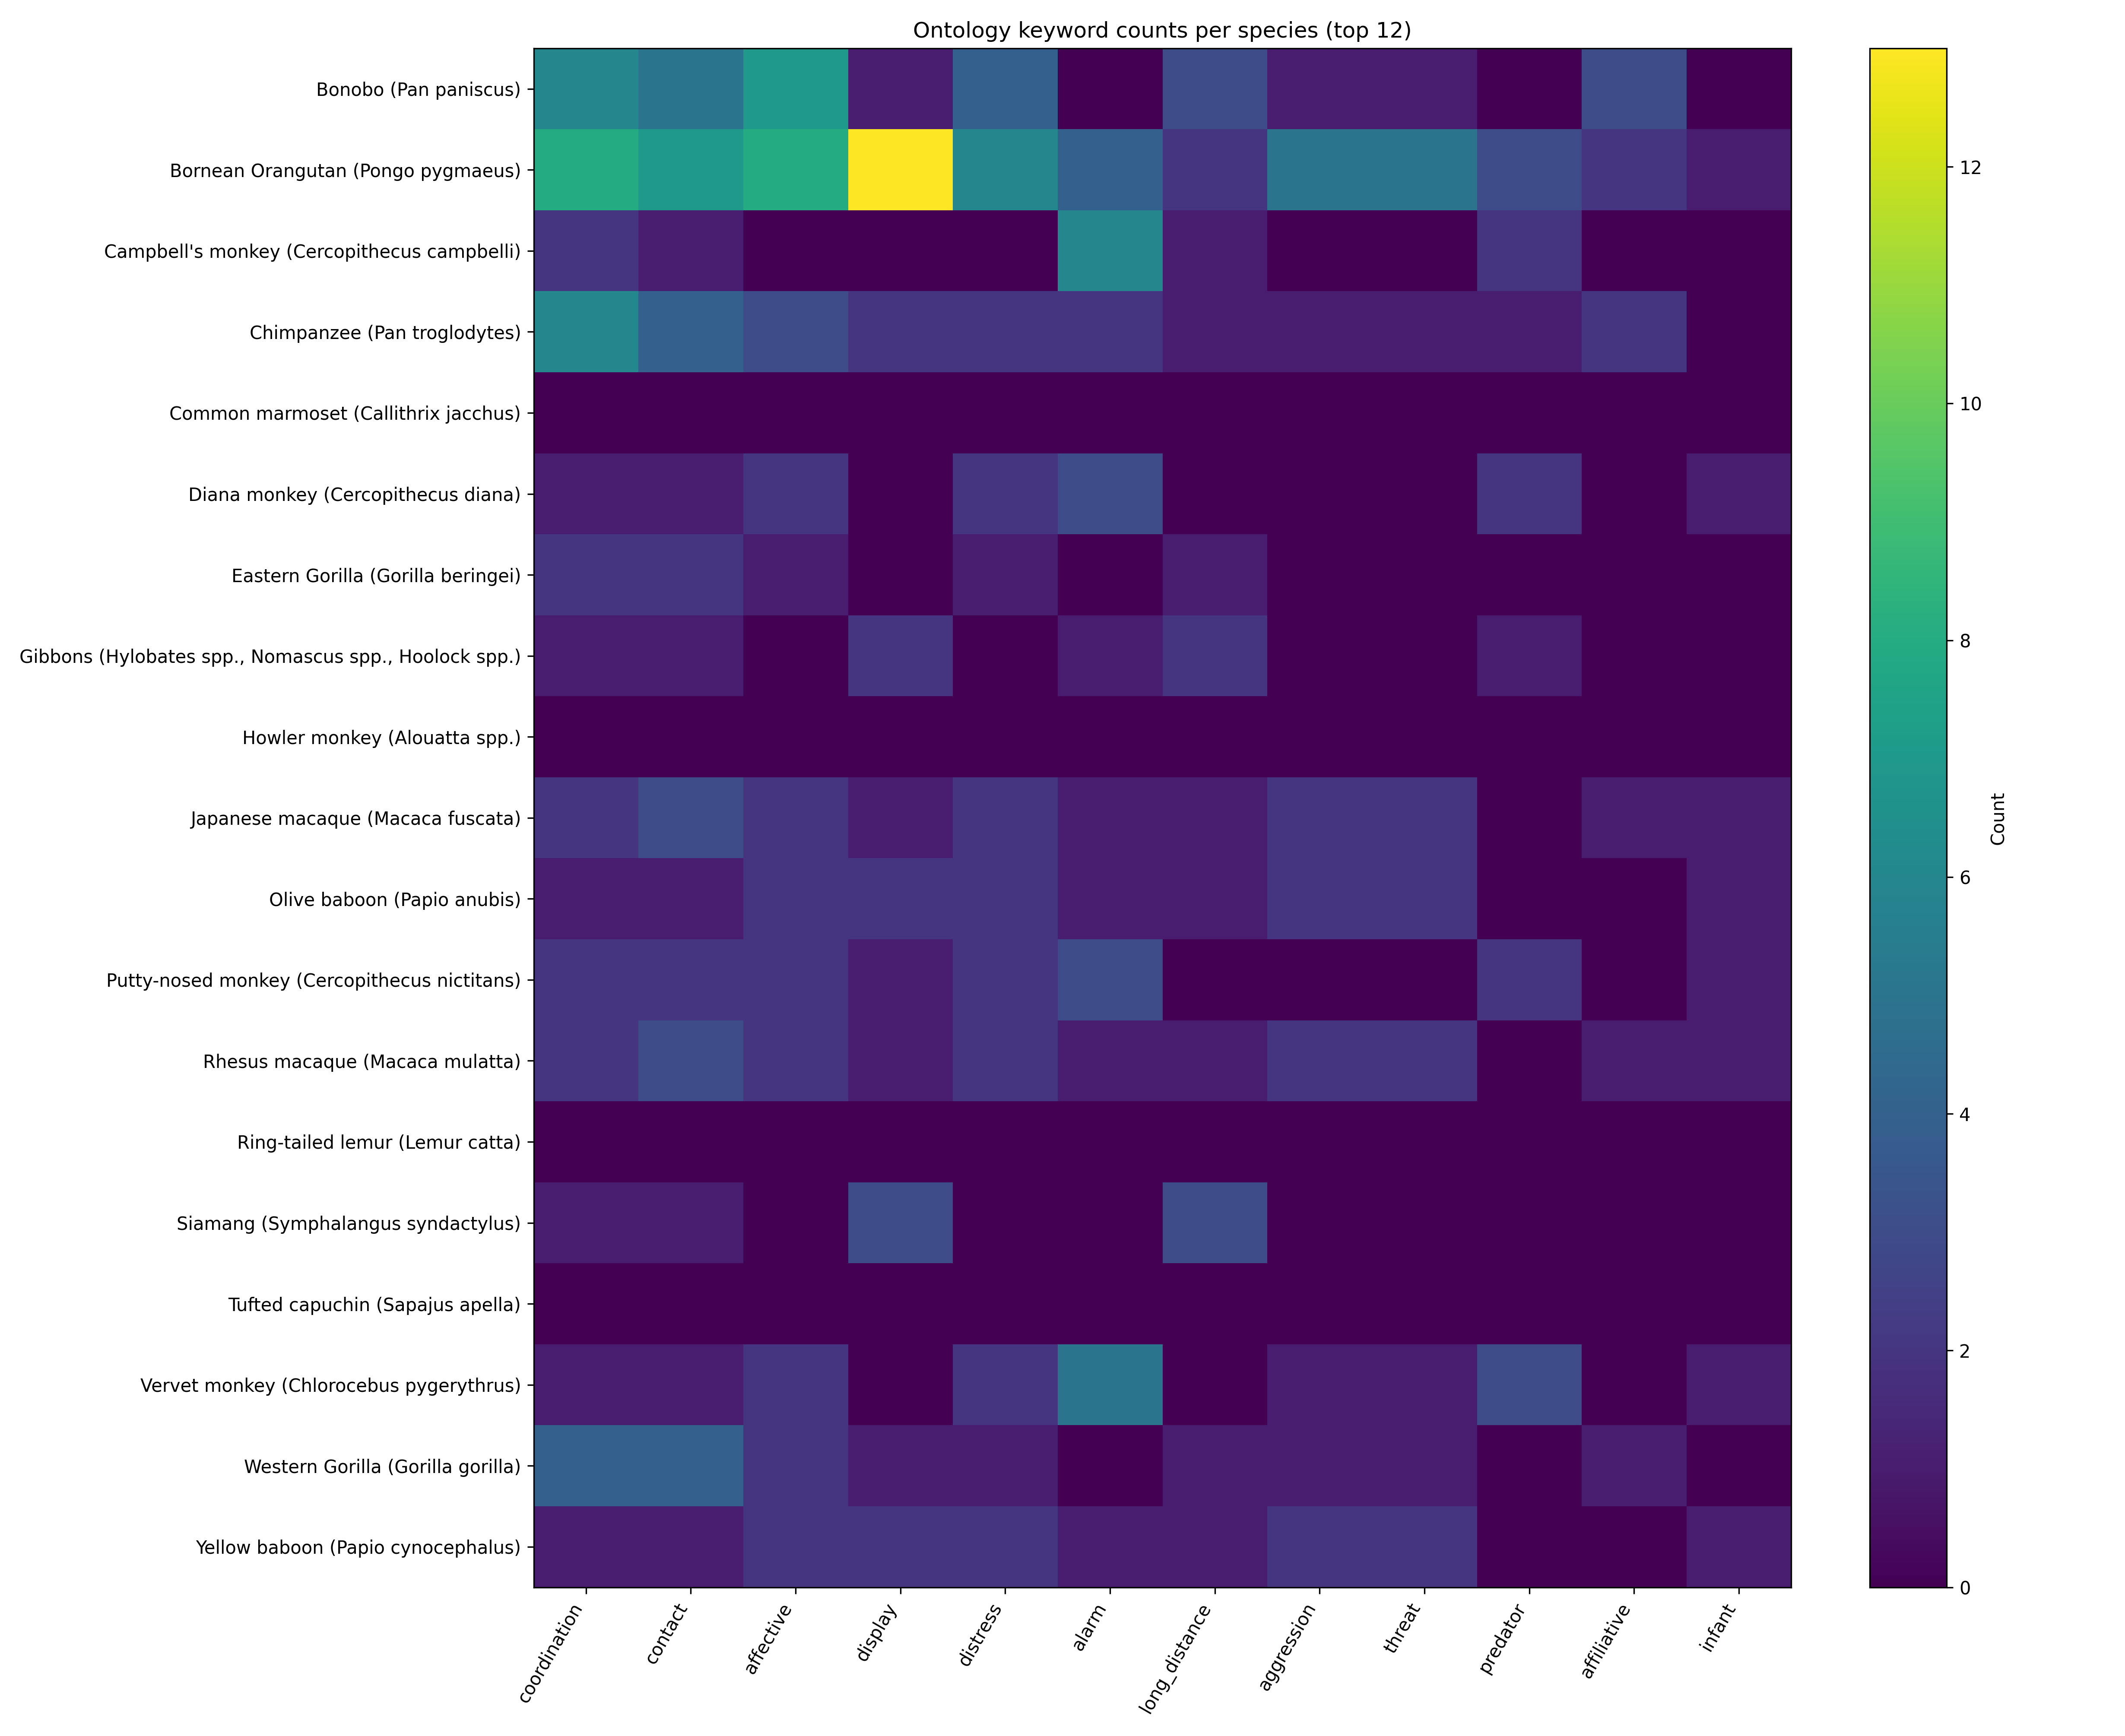
\includegraphics[width=\textwidth]{../plots/keyword_heatmap.png}
	\caption{\textbf{Form-to-meaning stability: correlational evidence.} (\textbf{A}) Pairwise acoustic distance vs.\ pairwise semantic distance for all call pairs in \dbname, with Mantel test statistics reported within and across species and taxa. Each point is a pair of calls; color indicates whether the pair is within-species, across-species within a taxonomic family, or across families. (\textbf{B}) Co-occurrence heatmap of semantic and acoustic ontology keywords, showing systematic associations (e.g., alarm calls are described as broadband and high-frequency; contact calls as tonal and low-frequency). [Placeholder: panel A awaits numeric results.]}
	\label{fig:mantel}
\end{figure}

The most direct test of form-to-meaning stability is whether calls that are acoustically similar are also semantically similar. We computed pairwise cosine distances in both the acoustic and semantic embedding spaces for all $\ncalls \times (\ncalls-1)/2 = 69{,}378$ call pairs in \dbname, and tested their correlation using the Mantel test \cite{mantel1967detection} with 10,000 permutations.

Across all call pairs, acoustic and semantic distances are significantly positively correlated ($r = [X.XX]$, $p < 0.001$; Figure~\ref{fig:mantel}A). This result holds within individual species ($r = [X.XX]$, $p < 0.001$), across species within the same taxonomic family ($r = [X.XX]$, $p < 0.001$), and even across species from different families ($r = [X.XX]$, $p < 0.001$). The correlation is strongest within species and weakens, but remains significant, across increasing taxonomic distances, suggesting that form-to-meaning mapping is most conserved within lineages but retains structure at the scale of the tree of life.

\subsection{Keyword co-occurrence analysis}

As a complementary, more transparent analysis, we examined the point-wise mutual information (PMI) between acoustic and semantic ontology keywords across all calls. Several strong associations emerge (Figure~\ref{fig:mantel}B). Alarm calls---characterized semantically by keywords such as \textit{alarm}, \textit{predator}, and \textit{threat}---are disproportionately described acoustically as broadband, high-frequency, or short-duration. Contact calls (semantic: \textit{contact}, \textit{coordination}, \textit{long\_distance}) are more often described as tonal and repetitive. Infant-directed calls (semantic: \textit{infant}, \textit{distress}) are frequently described as high-pitched. These patterns are consistent with functional explanations: localizability and urgency for alarms, long-range propagation for contact, species-typical signal properties for parent-offspring communication.

\section{Result 2: Form-to-meaning stability---predictive evidence}

\subsection{Cross-generalization experiments}

Correlational evidence establishes that acoustic and semantic spaces are aligned in \dbname, but does not test whether this alignment supports prediction. We therefore trained a model to predict the semantic embedding of a call from its acoustic embedding, and evaluated its generalization under four hold-out conditions designed to test progressively more demanding forms of transfer:

\begin{enumerate}
	\item \textbf{Within-repertoire}: hold out random calls from species present in training.
	\item \textbf{Across species}: hold out all calls from a subset of species.
	\item \textbf{Across taxa}: hold out all calls from a subset of higher-level taxa (families or orders).
	\item \textbf{Across contexts}: hold out calls belonging to specific semantic categories (e.g., all alarm calls).
\end{enumerate}

\subsection{Model and evaluation}

The predictor maps from acoustic embedding space to semantic embedding space. We tested several architectures: (1) a linear regression (regularized via ridge penalty), corresponding to a rotation/rescaling of the acoustic space; (2) a shallow MLP; and (3) retrieval-based prediction, in which the predicted semantic representation is the average of the $k$ most similar training calls in acoustic space. Performance is evaluated by the cosine similarity between the predicted and true semantic embeddings, and by the rank of the true call's semantic embedding among all calls in the hold-out set (mean reciprocal rank, MRR).

\begin{table}[h]
	\centering
	\caption{\textbf{Form-to-meaning prediction across generalization conditions.} Mean cosine similarity (Cos.) and mean reciprocal rank (MRR) between predicted and true semantic embeddings, under four hold-out conditions. Higher is better. [Placeholder: values to be filled upon running experiments.]}
	\label{tab:prediction}
	\begin{tabular}{lcccccc}
		\toprule
		& \multicolumn{2}{c}{\textbf{Within-repertoire}} & \multicolumn{2}{c}{\textbf{Across species}} & \multicolumn{2}{c}{\textbf{Across taxa}} \\
		\cmidrule(lr){2-3}\cmidrule(lr){4-5}\cmidrule(lr){6-7}
		\textbf{Model}    & Cos. & MRR & Cos. & MRR & Cos. & MRR \\
		\midrule
		Random baseline   & ---  & --- & ---  & --- & ---  & --- \\
		Retrieval ($k=1$) & ---  & --- & ---  & --- & ---  & --- \\
		Linear (ridge)    & ---  & --- & ---  & --- & ---  & --- \\
		MLP               & ---  & --- & ---  & --- & ---  & --- \\
		\bottomrule
	\end{tabular}
\end{table}

Results are summarized in Table~\ref{tab:prediction}. Across all conditions, [to be filled: qualitative summary of results once computed]. The across-taxa generalization result is particularly notable: it suggests that the acoustic-semantic alignment in \dbname is not merely a product of within-lineage acoustic evolution, but reflects structural regularities that transcend phylogenetic boundaries.

\section{Result 3: Acoustic-semantic feature alignment (optional)}

\subsection{Hypothesis-driven analysis}

The correlational and predictive results above establish the existence and learnability of form-to-meaning mapping, but do not identify its structure. To gain mechanistic insight, we performed an ablation analysis: for each pair of acoustic keyword $a$ and semantic keyword $s$, we computed the PMI between $a$ and $s$ across all calls in \dbname, yielding a matrix of acoustic-semantic associations.

\begin{figure}[t]
	\centering
	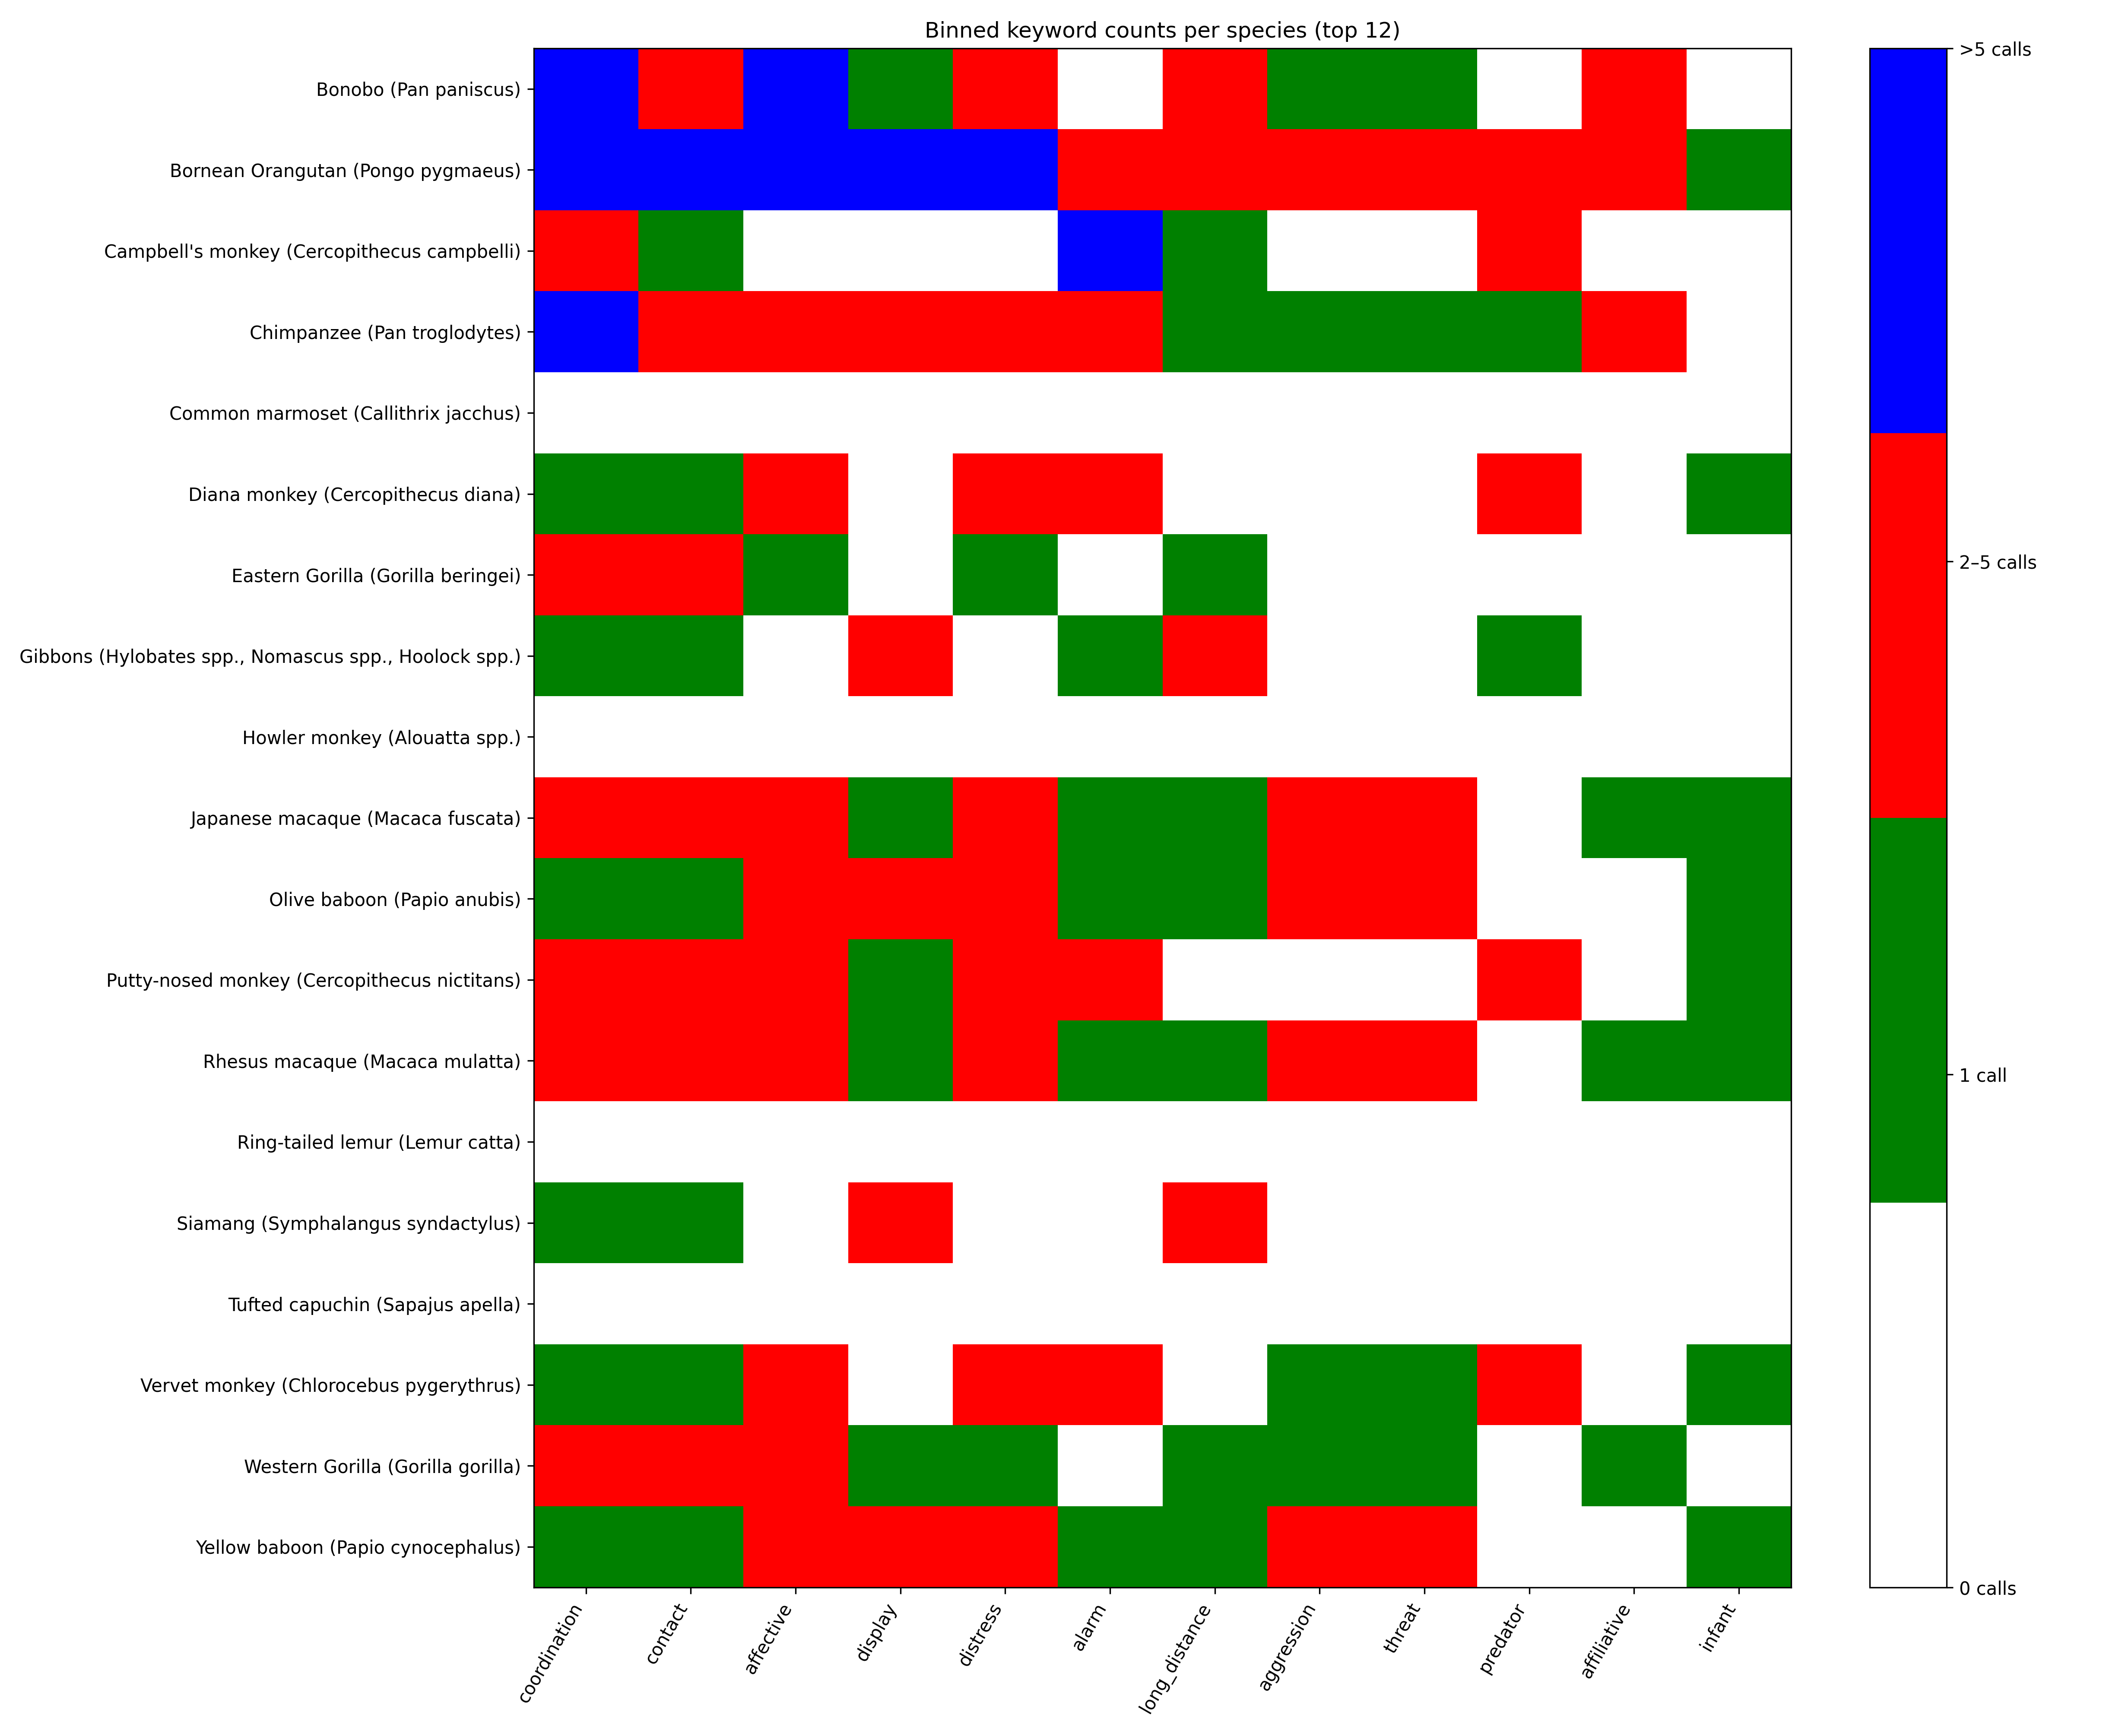
\includegraphics[width=\textwidth]{../plots/keyword_heatmap_bin.png}
	\caption{\textbf{Acoustic-semantic feature alignment.} PMI heatmap between acoustic and semantic ontology keywords. Positive values (dark) indicate that the acoustic feature is more common among calls with the given semantic function than expected by chance. Negative values (light) indicate anti-association.}
	\label{fig:pmi}
\end{figure}

Figure~\ref{fig:pmi} reveals several interpretable patterns. High-frequency acoustic features are most strongly associated with alarm and distress semantics. Tonal features co-occur with contact and affiliative semantics. Broadband or noisy features associate with aggression and threat. These associations are consistent with functional acoustic ecology hypotheses and with sound symbolism findings in human language research \cite{ohala1994sound}. The analysis provides a transparent, keyword-level decomposition of the form-to-meaning code identified in Results 1--2.

\section{Lexical translation}

\subsection{Translating human concepts to animal calls}

The form-to-meaning stability results motivate a direct application: given any human concept expressible in natural language, we can identify its closest animal-kingdom analogue by (1) embedding the concept in semantic space using the same sentence transformer, and (2) retrieving the call in \dbname whose semantic embedding is nearest. This constitutes a \emph{lexical translation} from human language into animal vocal repertoires.

Table~\ref{tab:translation} shows examples. Human words such as \textit{danger}, \textit{hunger}, \textit{greeting}, and \textit{territory} map to intuitively sensible animal calls: the anti-predator alarm calls of meerkats, the begging calls of nestlings, contact calls of elephants, and territorial advertisement calls of wolves. The translation is grounded in the entire corpus of documented animal vocalizations, representing the full state of scientific knowledge as compressed by language models.

\begin{table}[h]
	\centering
	\caption{\textbf{Lexical translation: selected examples.} For each human concept (left), we show the best-matching call in \dbname by semantic similarity (center), and its acoustic description (right). [Placeholder: to be filled once translation pipeline is complete.]}
	\label{tab:translation}
	\begin{tabular}{p{3cm}p{5cm}p{5cm}}
		\toprule
		\textbf{Human concept} & \textbf{Best-match call}  & \textbf{Acoustic description} \\
		\midrule
		danger                 & [species] --- [call name] & [acoustic description]        \\
		hunger                 & [species] --- [call name] & [acoustic description]        \\
		greeting               & [species] --- [call name] & [acoustic description]        \\
		come closer            & [species] --- [call name] & [acoustic description]        \\
		I am here              & [species] --- [call name] & [acoustic description]        \\
		\bottomrule
	\end{tabular}
\end{table}

\subsection{Extending beyond documented knowledge}

The retrieval approach is conservative: it is limited to calls for which we have semantic annotations in \dbname. We can extend it using the predictive model from Result 2: for calls not yet semantically documented, the model provides a best-guess semantic embedding from acoustic features alone. This enables translation not only for the \ncalls documented calls in \dbname, but for any acoustic recording that can be embedded in acoustic description space.

Together, these two modes---retrieval for documented calls, prediction for undocumented ones---constitute a scalable pipeline for cross-species lexical translation. We release a web application (\url{[placeholder URL]}) that allows users to explore the translation interactively.

\section{Discussion}

\subsection{Evidence for a biological code}

Our results suggest that the relationship between acoustic form and communicative meaning in animal vocalizations is not arbitrary. Acoustic and semantic distances are correlated across the tree of life, a predictive model trained on this relationship generalizes across species and taxa, and specific acoustic features are non-randomly associated with specific semantic functions. Taken together, these findings are consistent with the hypothesis that a biological code---a set of structural regularities linking form to meaning---is a widespread organizational principle of animal communication.

What could explain such a code? Two non-exclusive mechanisms are plausible. First, \emph{physical and environmental constraints} may channel the evolution of both acoustic form and communicative function in correlated ways. Short, broadband calls may be independently favored in multiple lineages for alarm signaling because they are easily localized and rapidly recognizable \cite{marler1955characteristics}; high-pitched calls may be independently favored for infant-directed signaling because of their arousing and attention-capturing properties \cite{ohala1994sound}. These convergent functional pressures would produce the acoustic-semantic associations we observe even in the absence of shared ancestry.

Second, \emph{common descent} may conserve acoustic-semantic associations within phylogenetic lineages. Calls and their associated meanings may evolve slowly, such that the form-to-meaning mapping documented in an ancestral species is partially preserved in descendants. This would explain why form-to-meaning correlations are strongest within species and within families, and weaker---though still significant---across more distant taxa.

Disentangling these mechanisms will require more extensive phylogenetically controlled analyses, ideally combined with audio data that can be directly analyzed without reliance on textual descriptions. Our current dataset, which is built from textual annotations, is a first step; future work should integrate acoustic features extracted directly from recordings.

\subsection{Limitations and future directions}

Several limitations deserve explicit acknowledgment. First, \dbname is built from textual descriptions of calls, not from audio. The acoustic embeddings we use are therefore embeddings of \emph{descriptions of sounds}, not of the sounds themselves. This means that our form-to-meaning results are contingent on the quality and consistency of the descriptions, and on whether the features that are saliently described are the same as those that carry communicative information. Future work should test whether form-to-meaning structure replicates when acoustic representations are derived directly from audio (e.g., using models such as AVES~\cite{hagiwara2022avesanimalvocalizationencoder} or NatureLM-audio~\cite{robinson2025naturelmaudio}).

Second, \dbname is taxonomically skewed toward well-studied mammalian species, particularly species that have been the subject of detailed ethological and cognitive studies (elephants, primates, cetaceans). Birds and amphibians are underrepresented. Expanding the database to cover a broader and more balanced taxonomic sample is a high priority.

Third, the semantic ontology we use, while designed to be broadly applicable, is necessarily human-derived. The categories \textit{alarm}, \textit{contact}, \textit{affective}, and \textit{coordination} are useful but coarse; many calls carry meaning that does not map cleanly onto these dimensions. Developing richer, more species-sensitive semantic representations is an open challenge.

Finally, our translation results should be interpreted carefully. The claim is not that animals \emph{have} the concept corresponding to a given human word, but that their vocalizations, as documented in the scientific literature, are semantically closest to that word as measured by embedding similarity. Translation is a first approximation, not a claim of cognitive equivalence.

\section{Conclusion}

We have introduced \dbname, a curated cross-species repertoire database, and used it to demonstrate that acoustic form and communicative meaning are systematically related across the animal kingdom. This form-to-meaning stability is strong enough to support prediction and cross-species translation. Our results suggest that the accumulated knowledge of comparative ethology---as compressed and structured by large language models---is sufficient to begin answering questions about communication at the scale of the tree of life. We hope that \dbname, and the methods we introduce, will serve as a foundation for a new generation of large-scale, comparative, and translational bioacoustics.

% ------------------------------------------------------------------ %
%  CONTRIBUTIONS
% ------------------------------------------------------------------ %
\section{Contributions}
{\small\hyphenpenalty=10000
{\headingfont Conceptualization:} A.B., C.D.
{\headingfont Methodology:} A.B., C.D., E.F.
{\headingfont Software:} E.F., G.H.
{\headingfont Validation:} C.D., E.F.
{\headingfont Formal analysis:} A.B., E.F.
{\headingfont Investigation:} A.B., C.D.
{\headingfont Resources:} I.J.
{\headingfont Data curation:} A.B., C.D., E.F.
{\headingfont Writing -- original draft:} A.B.
{\headingfont Writing -- review \& editing:} A.B., C.D., E.F., I.J.
{\headingfont Visualization:} E.F., G.H.
{\headingfont Supervision:} I.J.
{\headingfont Project administration:} I.J.
{\headingfont Funding acquisition:} I.J.}

\section{Acknowledgements}
We thank the researchers whose detailed ethological and bioacoustic studies form the foundation of \dbname.

% ------------------------------------------------------------------ %
%  REFERENCES
% ------------------------------------------------------------------ %
\clearpage
\printbibliography
\clearpage

% ------------------------------------------------------------------ %
%  SUPPLEMENTARY INFORMATION
% ------------------------------------------------------------------ %
\setcounter{section}{0}
\renewcommand{\thesection}{\Alph{section}}

\section{Supplementary Information}

\subsection{Web application}

We release a web application at \url{[placeholder URL]} that allows users to:
\begin{enumerate}
	\item Browse the full \dbname database, filtered by species, taxonomic group, or semantic category.
	\item Perform lexical translation: enter a human concept and retrieve the closest animal calls.
	\item Perform reverse translation: select a call and retrieve the closest human semantic descriptions.
	\item Explore the semantic and acoustic embedding spaces interactively via UMAP projection.
\end{enumerate}

\subsection{Full database statistics}

\begin{figure}[h]
	\centering
	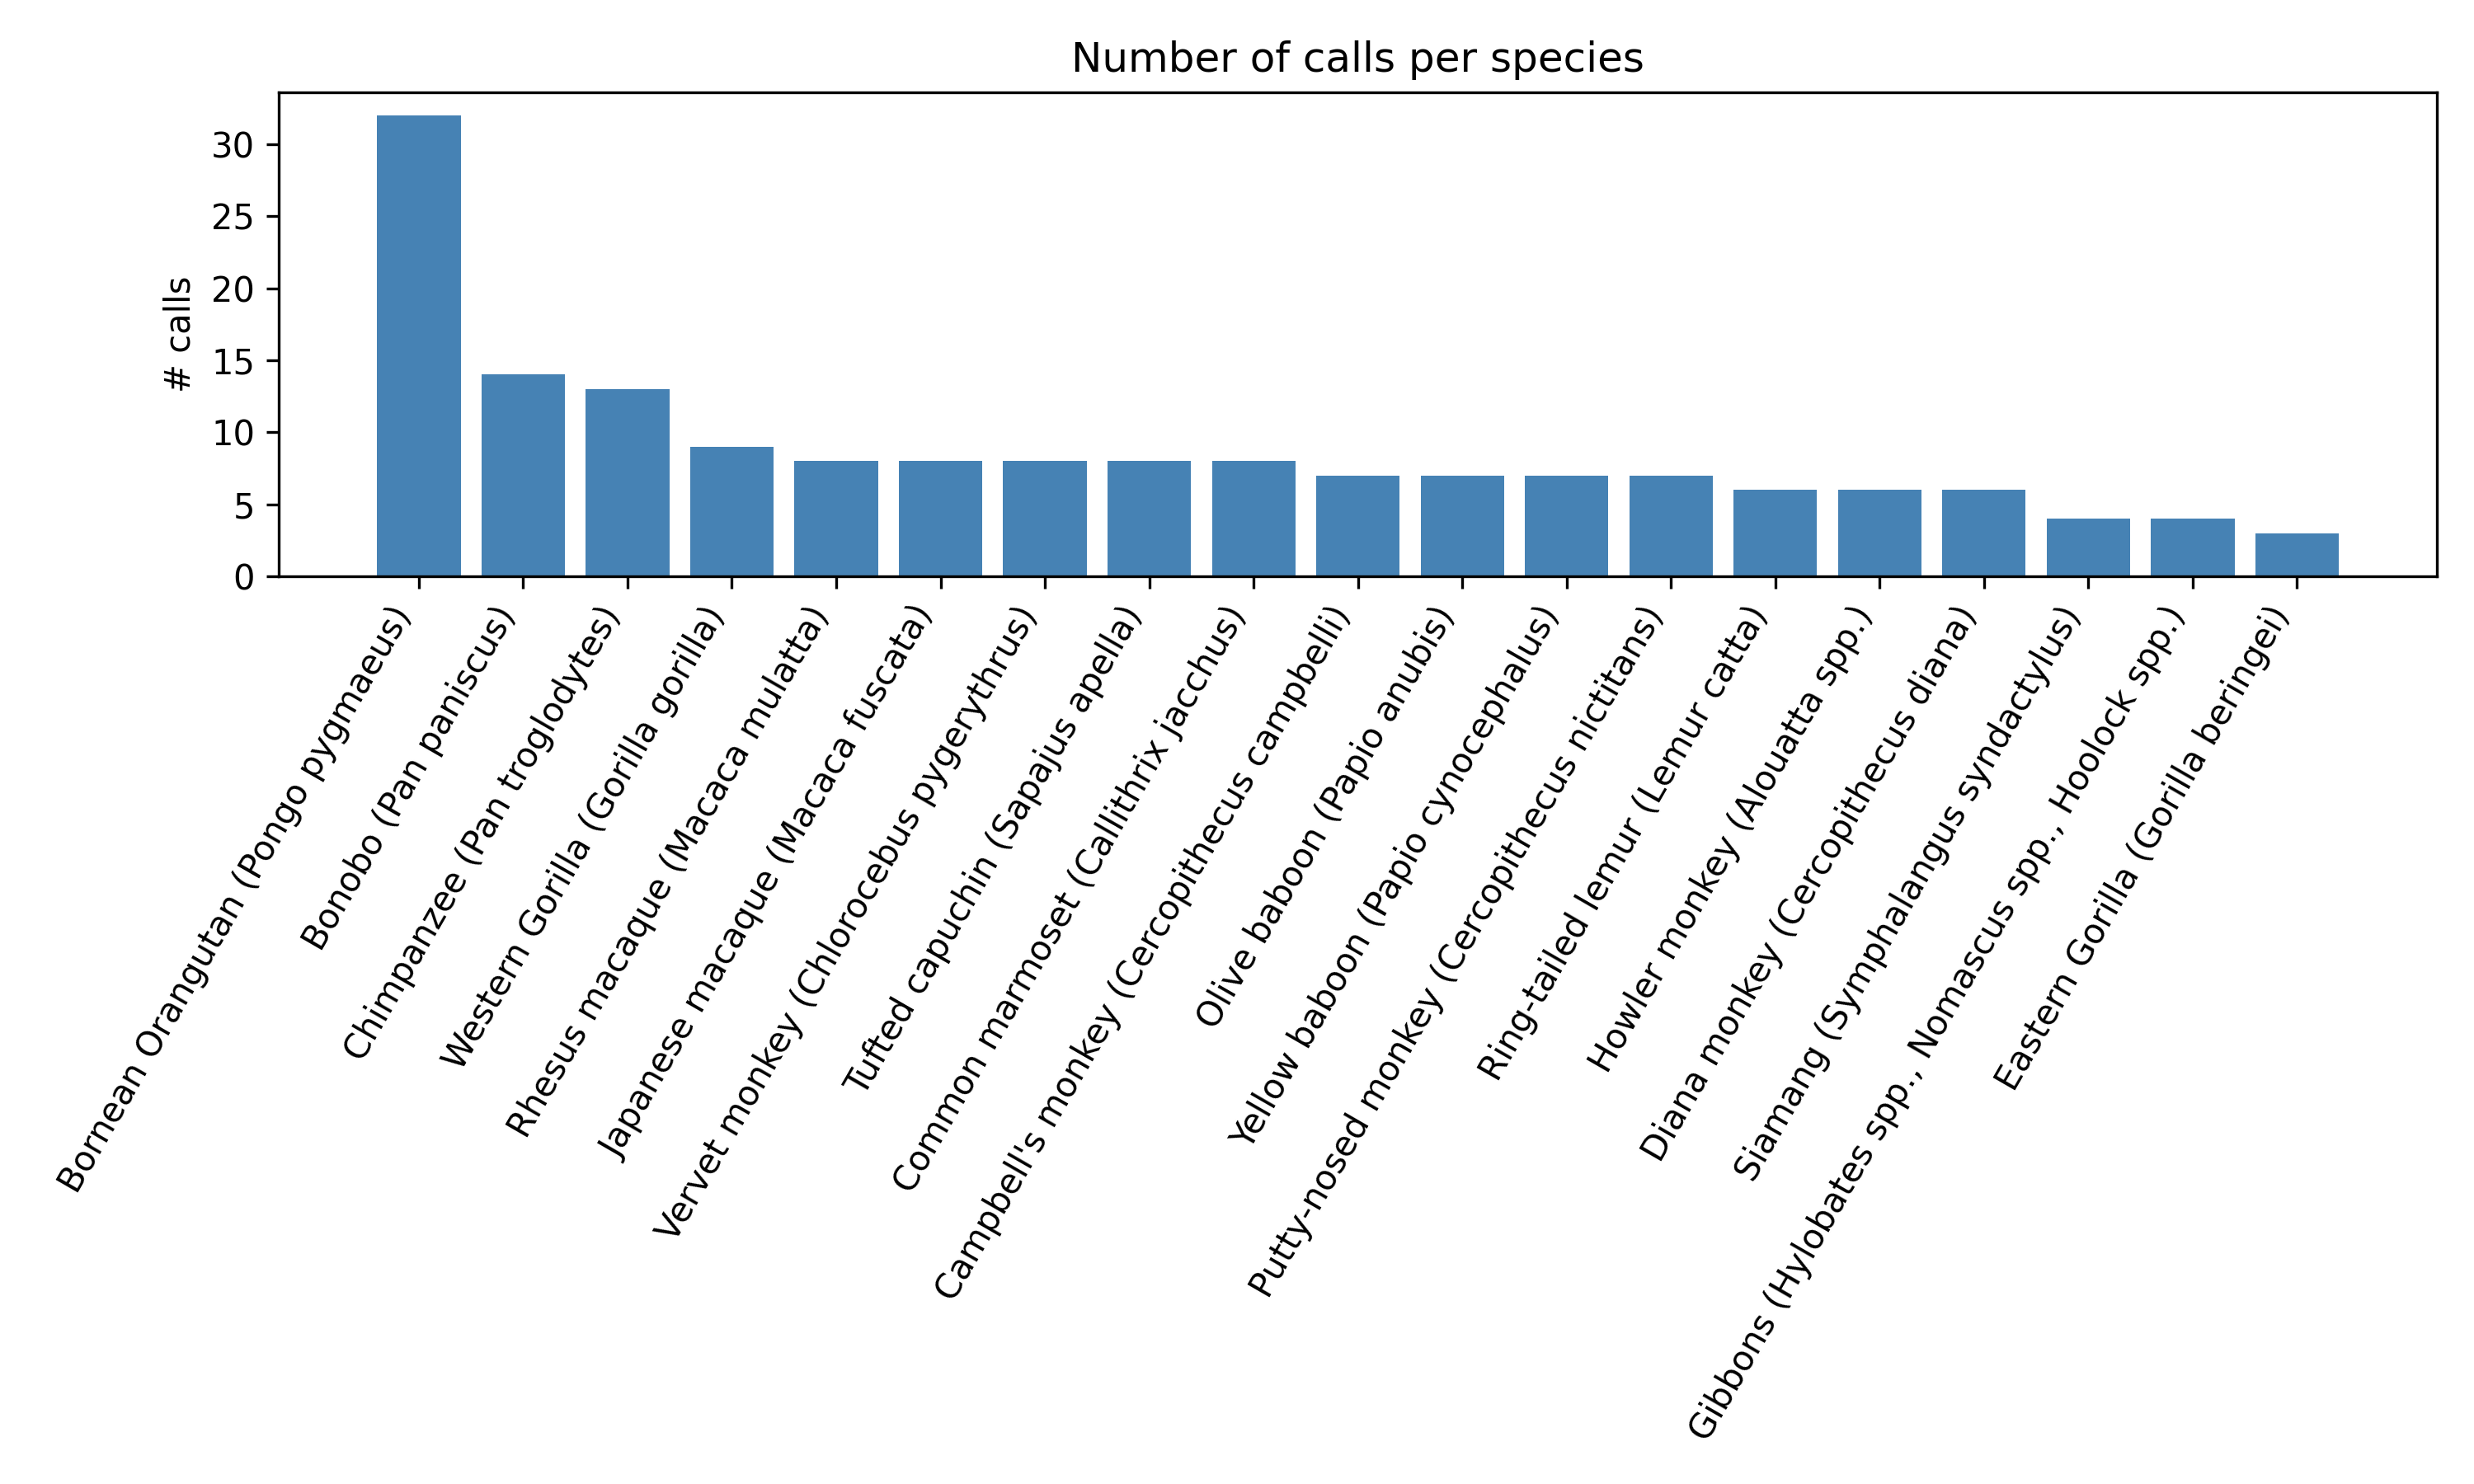
\includegraphics[width=\textwidth]{../plots/calls_per_species.png}
	\caption{\textbf{Calls per species in \dbname.} Each bar represents one species; color encodes taxonomic class.}
	\label{fig:calls_per_species}
\end{figure}

\begin{figure}[h]
	\centering
	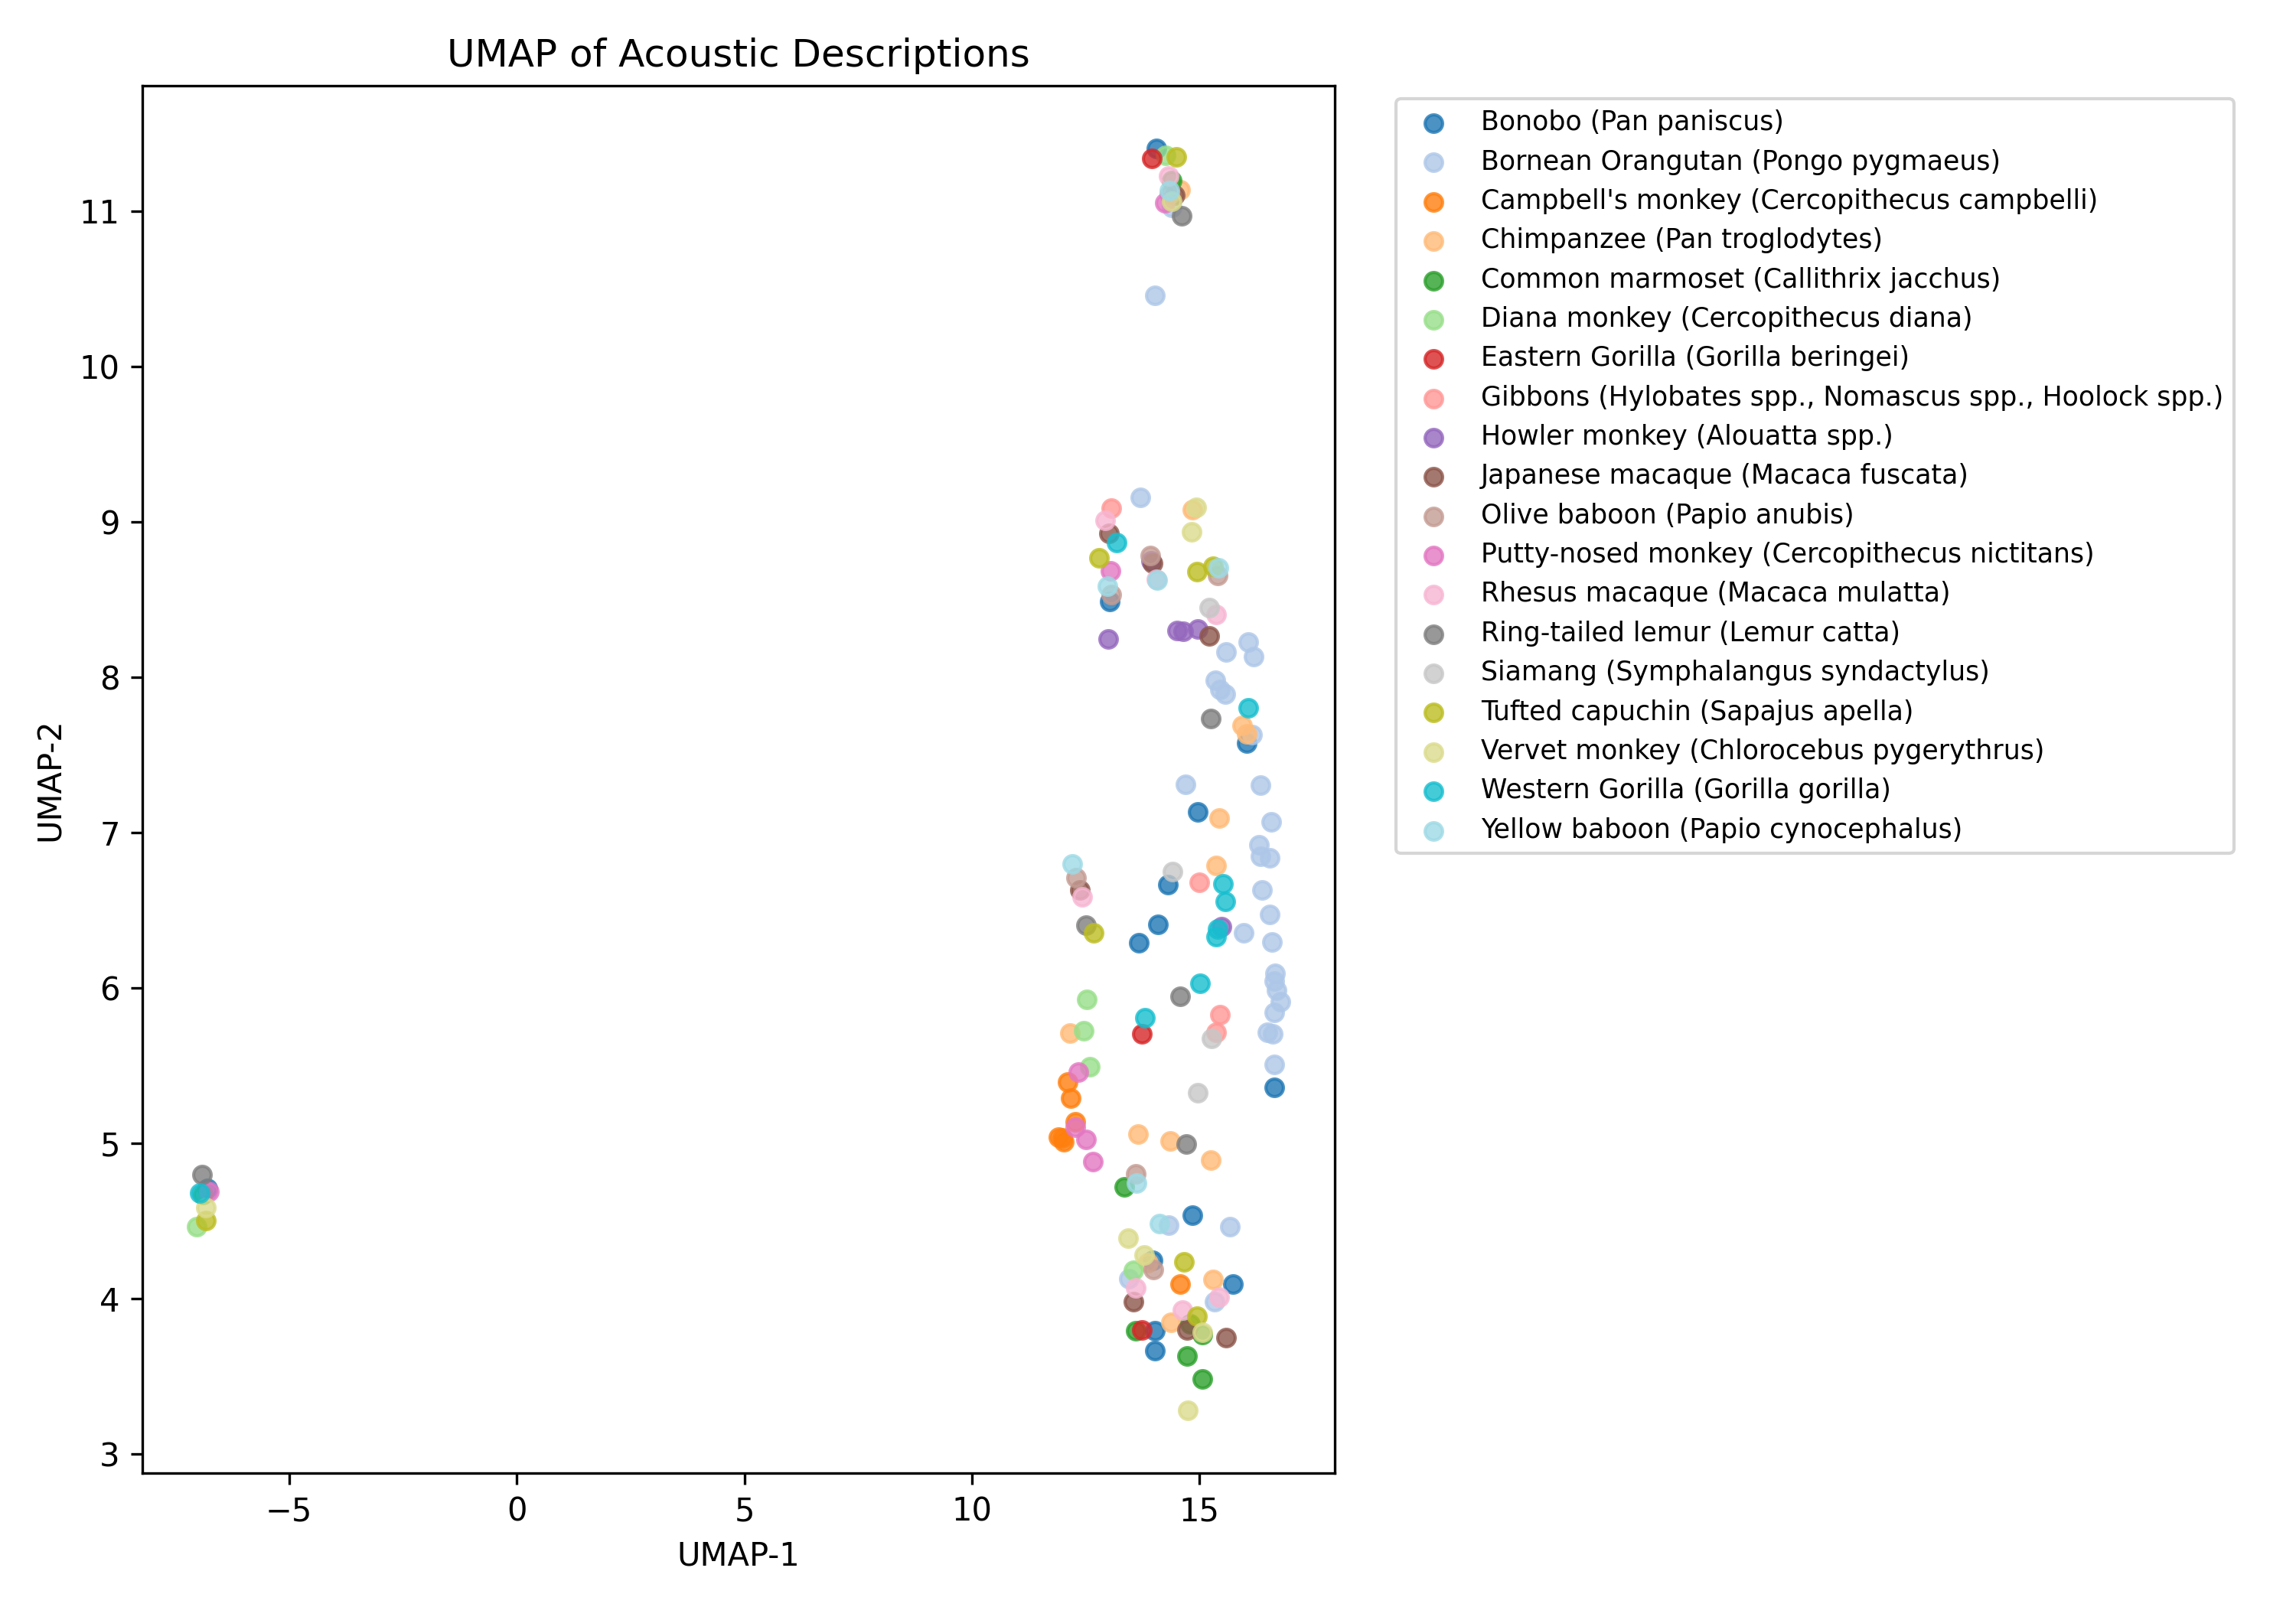
\includegraphics[width=0.8\textwidth]{../plots/acoustic_umap.png}
	\caption{\textbf{Acoustic embedding space (UMAP).} Each point is a call, colored by taxonomic class. Calls with acoustically similar descriptions cluster together.}
	\label{fig:acoustic_umap}
\end{figure}

\end{document}
